\documentclass{article}
\usepackage[style=apa]{biblatex}
\addbibresource{NLP-entailment.bib}
\usepackage{graphicx}
\graphicspath{{./Images}}
\usepackage{algpseudocode}
\usepackage{tcolorbox}
\usepackage{array}
\usepackage{svg}
\usepackage{hyperref}

\author{Hynek Kydlíček}
\title{Seq to seq approach to entailment problem}
\begin{document}
    \maketitle
    \begin{abstract}
        In this paper we will be looking at Natural language inference problem.
        Precisely we will evaluate seq to seq approaches to this problem.
    \end{abstract}

    \section{Introduction}


    \subsection{Natural language inference}
    Natural language interface problem also called entailment problem is a problem of determining whether a given sentence is entailed by another sentence.
    One ordered pair (S1, S2) of sentences can be either contradiction, neutral or entailment.
    \begin{enumerate}
        \item A pair is entailment if second is implied by first sentence.\\
            Example:
            \begin{quotation}
                S1: `My brother's name is Hynek'
            \end{quotation}
            \begin{quotation}
                S2: `I have a brother'
            \end{quotation}

        \item A pair is contradiction if second sentence in contradiction with first sentence.\\
            Example:
            \begin{quotation}
                S1: `I have one brother, his name is Hynek'  
            \end{quotation}
            \begin{quotation}
                S2: `I have a brother called Peter'
            \end{quotation}

        \item A pair is neutral if pair is neither entailment nor contradiction.\\
            Example
            \begin{quotation}
                S1: `I have a brother'
            \end{quotation}
            \begin{quotation}
                S2: `I have a sister'
            \end{quotation}
    \end{enumerate}
    While the description is simple, the problem is not and there are few things that need to be considered.
    \begin{enumerate}
        \item Different languages problem: The sentences can be in different languages.
        \item Entity coreference problem: Given two sentence: S1: `Peter slept at home', S2: `Peter slept at his friends' it is not clear if both sentences refer to the same Peter
        \item Events coreference problem: Given two sentence: S1: `I am in library', S2: `I am in school' it is not clear whether both events are happening at the same time.
    \end{enumerate}
    Due to these problems we decided to use dataset which tackles these problems.

    \subsection{SNIL dataset}
    SNIL dataset was created at Stanford University and is a collection of 570k sentence pairs (\cite{StanfordNaturalLanguage}).
    It was introduced in 2016 and is one of the most popular dataset for NLI problem.
    The sentences are in English and are annotated by humans. The collection of data was done by crowdsourcing with Amazon Mechanical Turk.
    The crowdsourcers were given a image caption from Flickr which served as a premise and they had to write a sentence which would be either in contradiction, neutral or entailment relation with the premise.
    The mentioned problems were solved by
    \begin{enumerate}
        \item Different languages problem: All sentences in English.
        \item Entity coreference problem: The image captions grounded the sentence to specific situation and the participants had to make sentence with respect to the situation.
        \item Event coreference problem: Same as above
    \end{enumerate}
    The sentences were then validated by another group of humans and only ones with high inter-annotator agreement were kept.
    The paper by~\cite{bowmanLargeAnnotatedCorpus2015} that introduced the dataset also introduced a SOTA model of that time with accuracy of 80.8\% on test set.
    \subsection{Seq to seq problem and approaches}
    Seq to seq problem is a problem of translating one sequence to another. The most typical example is translating from one language to another.
    The problem is usually solved by using encoder-decoder architecture. The first sequence is first encoded into a context vector and the context vector decoded into the second sequence.
    There are two prominent deep learning approaches that emerged in the last few years RNNs and Transformers.
    \subsubsection{RNNs}
    RNNs are a type of neural network that can be used to solve seq to seq problem.
    From overview they look like Figure~\ref{fig:rnn}.
    \begin{figure}[h!]
        \centering
        \includegraphics[width=0.5\textwidth]{architecture-rnn-ltr.png}
        \caption{RNN architecture~(\cite{CS230Recurrent})}
        \label{fig:rnn}
    \end{figure}
    
    The problem of RNNs is that they are not able to capture long term dependencies.
    They are also not able to parallelize the computation because they depend on previous context vector.
    There is also a problem of vanishing gradient which makes it hard to train RNNs.
    The vanishing gradient is partially solved by using LSTM and GRU cells.
    The LSTM cells are very similar to standard RNN cell but have one more vector they pass between each other called cell state.
    This helps with gradient propagation.~\cite{staudemeyerUnderstandingLSTMTutorial2019} is a good in-depth look at LSTM cells.

    

    \subsubsection{Transformers}
    Transformers are newer architecture that was introduced in 2017 by~\cite{vaswaniAttentionAllYou2017b}.
    The overview of architecture can be seen at Figure~\ref{fig:transformer}.
    \begin{figure}[h!]
        \centering
        \includegraphics[width=0.5\textwidth]{attention.png}
        \caption{Transformer architecture~(\cite{vaswaniAttentionAllYou2017b})}
        \label{fig:transformer}
    \end{figure}
    The only part we will explain here is the multi-head attention as it's the most important one.
    If you are interested in more in-depth look at transformers please look at the paper.
    In input of multi-head attention we have $n$ vectors of size $d$. The vectors are translated into their 3 new representations Keys, Values and Queries.
    One Query is then dot-producted by every Key. The result is then softmaxed to normalize and then multiplied by appropriate Values.
    Then we sum results to get the vector of size $d$. We do this for every Query.
    This yields the same output size as input size. We can think of this as each input attending to all other inputs to find the most important ones (They will have high dot-product and thus they will impact the resulting vector the most).
    The attention can be done multiple time for one layer. This is why it's called multi-head.

    The encoder thus uses several layers of multi-head attention at the end producing k Keys and Values.
    The decoder also uses the multi-head attention with Queries,Keys and Values produced by input vectors but it also uses one
    where Keys and Values are ones produced by encoder and Queries are the ones produced by decoder.

    \subsection{Transfer learning}
    Transfer learning refers to technique of training a model on one task and then reusing the same model and it weights on another task.
    This can mean replacing the last layer of a model with a new one and training it on the new task while freezing the other layers or it can simply mean using the pretrained embeddings for the words and using the embeddings with the model
    In our case we will be using the second approach. We will train all our models with the Glove embeddings as defined in~\cite{penningtonGloVeGlobalVectors2014}.
    Glove embeddings is a collection of word embeddings.
    They exist in different variants varying in size and training corpus.
    We will be using the 300 dimensional 6B variant.


    \section{Methodology}
        \subsection{Research question}
        With all the key terms introduced we can now formulate our research question.
        \begin{quote}
            \textbf{We want to evaluate which of our trained models (RNN and Transformer) will have better accuracy on SNIL test dataset.}
        \end{quote}
        We chose these models to have at most 2M trainable parameters and we also required them to use 300d 6B Glove embeddings.
        We decided to use pretrained embedding because we wanted to focus on the architecture and not the embeddings. We also hopped that the embeddings would overall increase the accuracy of trained models as they carry implicit information.
        The 2M parameter limit was chosen to guarantee reasonable training time.

        \subsection{Hypothesis}
        Let's formulate the hypothesis:
        \begin{quote}
            \textbf{We predict that the Transformer model will have higher accuracy than the RNN model on SNIL test dataset.}
        \end{quote}
        To prove that we we will try to reject the null hypothesis, which can be stated as:
        \begin{quote}
            \textbf{The accuracy of the Transformer model will be less or equal than the accuracy of the RNN model on SNIL test dataset.}
        \end{quote}
        We chose the p-value of 0.05 as the threshold for rejecting the null hypothesis.
        We will use paired-bootstrap test to reject the null hypothesis.

    \section{Models description}
    In this section we will describe the RNN and Transformer models we trained.

    \subsection{RNN}
    For RNNs we decided to use simple LSTM multilayer cells.
    The multilayer version of LSTM cell is similar to the standard LSTM cell but it uses multiple LSTM cells at once.
    The input to next layers of cells is output from previous one. It was first introduced by~\cite{gravesSpeechRecognitionDeep2013}.
    Also there is a dropout layer between each layer of multilayer-LSTM cells.
    The architecture of the model can be seen at Figure~\ref{fig:rnn_model}.\\
    \begin{figure}[h!]
        \centering
        \includegraphics[width=0.5\textwidth]{LSTM.png}
        \caption{RNN model architecture}
        \label{fig:rnn_model}
    \end{figure}
    As can be seen we used max pooling to get vector for linear layer.
    We haven't tried other ways but it might be interesting to see, how other methods would evaluate (for examples sum).
    Also note that we used outputs of LSTM to feed into linear layer and not the hidden state.
    We tried using the hidden state but we got worse results.
    Total number of trainable parameters of this model is 1.8M.

    \subsection{Transformer}
    For transformer we tried many different architectures and we had really huge problems to get it trained.
    The biggest problem was that it was not overfitting even on one batch after 200 epochs.
    That is a problem as it shows model's inability to learn just hundreds (one batch) of samples.
    We tried to use just encoder with similar input and output processing as with RNNs but it didn't overfit even after 1k epochs.
    At the end we used the encoder decoder architecture. While it was also overfitting very slowly at least it was overfitting.
    The final architecture can be seen at Figure~\ref{fig:transformer_model}.
    \begin{figure}[h!]
        \centering
        \includegraphics[width=0.5\textwidth]{Transfomer.png}
        \caption{Transformer model architecture}
        \label{fig:transformer_model}
    \end{figure}

    Again we used max pooling to get vector for linear layer.
    Total number of trainable parameters is 1.9M.


    \subsection{Notes on training}
    \begin{enumerate}
        \item \textbf{We used Cross-entropy loss for both models.}\\
            We chose this loss as it is the most common one for classification tasks.
        \item \textbf{We used Adam optimizer with learning rate of 0.001 for both models.}\\
            We tried using different ($10^{-4}, 10^{-2}, 10^{-1}$) learning rates but we got worse loss after one epoch of training on test set.
            However we acknowledge that we should have used more sophisticated methods like (\cite{smithCyclicalLearningRates2017}).
        \item \textbf{We used gradient clipping with value of 0.5 for both models.}\\
            This was added mainly to prevent exploding gradients in RNNs.

        \item \textbf{We used 40 epochs for Transformer model and 20 epochs for RNN model.}\\
            These values were chosen to achieve reasonable training times.

    \end{enumerate}
    The training was done on K80 GPU with 12GB of memory on Google Colab (Because it's impossible to use school computers).
    All the code is available at \url{guess.ipynb} and is written in PyTorch.
    The trained model weights are available at \url{models/}.
    Tensorboard logs are available at \url{logs/}.


    \section{Results}
    The results of the models can be seen at Table~\ref{tab:results}.
    \begin{table}[h!]
        \centering
        \begin{tabular}{ | m{5em} | m{2cm}| m{3cm} | } 
            \hline
            Model & RNN & Transformer \\
            \hline
            Parameters & 1.8M & 1.9M \\
            \hline
            Accuracy (Train) & 0.96 & 0.7 \\
            \hline
            Accuracy (Test) & 0.78 & 0.69 \\
            \hline
        \end{tabular}
        \caption{Results of the models}
        \label{tab:results}
    \end{table}
    It's important to note that the dataset is well-balanced so the accuracy is a good metric to use.
    While the accuracy is way better than random chance model which would have $0.3$ accuracy, we were hoping to get better results for both models.
    The accuracy of the RNN is more than $20$ percent points higher than the accuracy of the Transformer on train dataset.
    As we said we had problems with inability to learn of the Transformer model and this is just another proof of that.
    The results on test dataset look a bit better for the Transformer model but it's still significant difference of 9 percent points.
    Overall difference is very dramatic on both datasets.
    The loss curves can be seen at Figure~\ref{fig:loss_curves}.
    The accuracy on training set can be seen at Figure~\ref{fig:acc_curves}.
    \begin{figure}[h!]
        \centering
        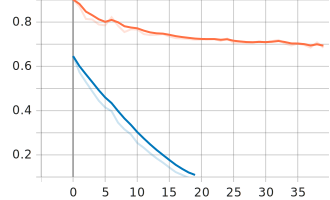
\includegraphics[width=0.5\textwidth]{Loss.png}
        \caption{Loss curves of the models}
        \label{fig:loss_curves}
    \end{figure}
    \begin{figure}[h!]
        \centering
        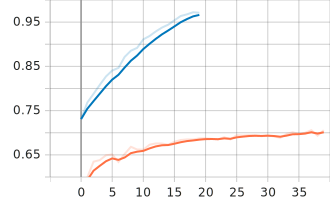
\includegraphics[width=0.5\textwidth]{Accuracy.png}
        \caption{Accuracy curves of the models}
        \label{fig:acc_curves}
    \end{figure}
    We tried to reject null-hypothesis with paired-bootstrap test and we got p-value of $1.0$.
    Thus we cannot reject the null-hypothesis and we can't say that our hypothesis is true with 95\% confidence.

    \section{Discussion}
    We were very surprised by the results. We expected the Transformer to perform much better, because
    of the attention mechanism. Clearly there was a problem with learning as we mention that we found it very hard
    to overfit on single batch and it was overall unstable. It might be solved by using different optimizer or scheduler. We don't think we could find
    a better loss function for this problem. It's also possible that the glove embeddings are not the best choice for this problem.

    Note: I talked about this with might bc. thesis supervisor and he said that I should have used leraning scheduler as the transformer need high learning rate at the beginning and then it should be decreased.
    Also he said that I should have used different optimizer as Adam is not the best choice for transformer.

    \section{Conclusion}
    We have evaluated the Transformer and RNN architecture on the NLI problem.
    While we expected the Transformer to perform much better, it didn't. However we could clearly see that it was generalizing way better.
    So it's possible that if we would substantially increase the number of parameters it would perform better. This would be very interesting to research in future.
    Another interesting thing would be to not use pretrained embedding but to train them. Last but not least we could try to fine-tune a language model for this task.


    \printbibliography{}
\end{document}